\documentclass{article}
\usepackage{tikz}

\begin{document}

\begin{figure}[h]
    \centering
    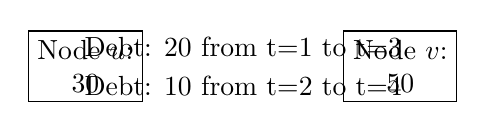
\begin{tikzpicture}[node distance=2cm, auto]
        % Define styles for nodes and edges
        \tikzset{
            node/.style={draw, rectangle, align=center},
            edge/.style={->, thick}
        }

        % Nodes
        \node[node] (u) at (0,0) {Node $u$: \\ \textup{\euro}30};
        \node[node] (v) at (4,0) {Node $v$: \\ \textup{\euro}50};

        % Edges with labels
        \path[edge] (u) -- node[midway, above] {Debt: \textup{\euro}20 from t=1 to t=3} (v);
        \path[edge] (v) -- node[midway, below] {Debt: \textup{\euro}10 from t=2 to t=4} (u);

    \end{tikzpicture}
    \caption{Simple Instance of the Interval Debt Model (IDM)}
    \label{fig:idm_example}
\end{figure}

\end{document}